\documentclass[aspectratio=169,10pt]{beamer}
\usepackage[utf8]{inputenc}
\usepackage[spanish,es-nodecimaldot]{babel}
\usepackage{amsmath,amssymb,amsfonts}
\usepackage{booktabs}
\usepackage{tabularx}
\usepackage{graphicx}

% Tema minimalista sin cajas ni decoraciones innecesarias
\usetheme{default}

% Unico color institucional para titulos, texto en negro estandar
\definecolor{maincolor}{RGB}{20, 45, 85}

\setbeamercolor{title}{fg=maincolor}
\setbeamercolor{frametitle}{fg=maincolor}
\setbeamercolor{structure}{fg=maincolor}
\setbeamercolor{normal text}{fg=black}

% Formato limpio de titulos
\setbeamertemplate{navigation symbols}{}
\setbeamertemplate{frametitle}{\vspace{0.3cm}\insertframetitle\par\vspace{0.1cm}\hrule\vspace{0.3cm}}
\setbeamertemplate{footline}[frame number]

\title{Optimizacion Cuadratica Multiperiodo de Portafolios\\Formulacion Determinista y Condiciones de Karush-Kuhn-Tucker (KKT)}
\subtitle{Del Modelo Original de Draviam a la Extension Regulatoria SFC en la BVC}
\author{Juan Mario Delgado Molina}
\institute{Curso de Optimizacion Lineal y Convexa\\Investigacion de Operaciones / Matematicas Aplicadas}
\date{Noviembre 2026}

\begin{document}

% SLIDE 1: PORTADA
\begin{frame}
  \titlepage
\end{frame}

% SLIDE 2: CONTEXTO Y LIMITACION DE MARKOWITZ
\begin{frame}{1. Contexto: De la Optimizacion de un Periodo al Enfoque Multiperiodo}
  En el modelo clasico de media-varianza de Markowitz (1952), la asignacion de recursos se optimiza para un unico horizonte de tiempo:
  \vspace{0.3cm}
  \begin{itemize}
    \item Se trata de un modelo estatico y miope, ya que ignora que un gestor financiero rebalancea su cartera en fechas intermedias sucesivas.
    \vspace{0.2cm}
    \item Optimizar periodo a periodo de forma independiente descarta la estructura de covarianza intertemporal entre activos en distintas fechas.
    \vspace{0.2cm}
    \item Esto genera costos transaccionales innecesarios y una trayectoria de rentabilidad sub-optima a lo largo del tiempo.
    \vspace{0.2cm}
    \item Para corregir esta limitacion, T. Draviam y T. Chellathurai (2002) formularon un modelo que optimiza de forma simultanea todas las decisiones de inversion a lo largo de un horizonte con multiples etapas.
  \end{itemize}
\end{frame}

% SLIDE 3: NATURALEZA DETERMINISTA DEL PROBLEMA
\begin{frame}{2. Naturaleza Determinista de la Formulacion}
  Aunque los precios en los mercados financieros evolucionan mediante procesos estocasticos continuos, el problema que se resuelve es puramente determinista:
  \vspace{0.3cm}
  \begin{itemize}
    \item Los momentos esperados y las covarianzas intertemporales se obtienen mediante formulas analiticas cerradas exactas basadas en la distribucion log-normal.
    \vspace{0.2cm}
    \item No se emplean simulaciones de Monte Carlo ni generadores aleatorios en tiempo de ejecucion.
    \vspace{0.2cm}
    \item Toda la informacion estocastica queda condensada previamente en un vector constante de precios esperados descontados $P$ y una matriz simetrica de covarianza intertemporal $C$.
    \vspace{0.2cm}
    \item En consecuencia, el problema a optimizar es un Programa Cuadratico (QP) continuo determinista con restricciones lineales, resoluble exactamente mediante condiciones KKT.
  \end{itemize}
\end{frame}

% SLIDE 4: ESPACIO DE DECISION
\begin{frame}{3. Espacio de Decision y Variables Primarias}
  El vector global de decisiones agrupa las asignaciones en las $M+1$ fechas de planeacion temporal $t_0, t_1, \dots, t_M$:
  \vspace{0.2cm}
  \begin{equation*}
    U = \begin{bmatrix} U_0 \\ U_1 \\ \vdots \\ U_M \end{bmatrix} \in \mathbb{R}^{(M+1)(N+1)}, \quad \text{donde cada } U_j = \begin{bmatrix} u_{0,j} \\ u_{1,j} \\ \vdots \\ u_{N,j} \end{bmatrix} \in \mathbb{R}^{N+1}
  \end{equation*}
  \vspace{0.2cm}
  Definicion de las variables de decision continuas:
  \begin{itemize}
    \item $u_{0,j}$: Proporcion de riqueza asignada al activo libre de riesgo (Titulos Soberanos TES) en la fecha $t_j$.
    \vspace{0.1cm}
    \item $u_{i,j}$: Proporcion invertida en la accion riesgosa $i$ ($i = 1, \dots, N$) en la fecha $t_j$.
    \vspace{0.1cm}
    \item Espacio de variables: Para $N$ acciones y $M$ etapas hacia adelante, el problema cuenta con $n = (M+1)(N+1)$ variables de decision primales.
  \end{itemize}
\end{frame}

% SLIDE 5: MODELO ORIGINAL DE DRAVIAM
\begin{frame}{4. El Modelo Original de Draviam y Chellathurai (2002)}
  En la formulacion original de Draviam y Chellathurai, el problema consiste en minimizar el riesgo global del portafolio penalizado por el retorno esperado:
  \vspace{0.3cm}
  \begin{equation*}
    \min_{U} \quad F(U) = -\theta' P^T U + \frac{1}{2} U^T C U
  \end{equation*}
  \vspace{0.2cm}
  sujeto a:
  \vspace{0.2cm}
  \begin{align*}
    A U &= b \quad &&\text{(Restricciones presupuestarias de igualdad en cada fecha)} \\
    U &\ge \mathbf{0} \quad &&\text{(No negatividad / Prohibicion de ventas en corto)}
  \end{align*}
  \vspace{0.2cm}
  Observacion: El modelo original no contempla cotas superiores de concentracion por emisor.
\end{frame}

% SLIDE 6: CONVEXIDAD EN EL MODELO ORIGINAL
\begin{frame}{5. Convexidad Estricta y Region Factible}
  Propiedades fundamentales del problema cuadratico:
  \vspace{0.3cm}
  \begin{itemize}
    \item Vector gradiente: $\nabla F(U) = -\theta' P + C U$.
    \vspace{0.1cm}
    \item Matriz hessiana: $\nabla^2 F(U) = C$.
    \vspace{0.1cm}
    \item La matriz de covarianza intertemporal $C$ es simetrica semidefinida positiva ($C \in \mathcal{S}_+^n$).
    \vspace{0.2cm}
    \item Al asegurar que el menor valor propio satisfaga $\lambda_{\min}(C) > 0$, la funcion objetivo $F(U)$ es estrictamente convexa.
    \vspace{0.2cm}
    \item La region factible esta definida por ecuaciones lineales ($AU = b$) y desigualdades de no negatividad ($U \ge \mathbf{0}$), formando un conjunto convexo acotado por la suma presupuestaria.
    \vspace{0.2cm}
    \item En un problema estrictamente convexo con region factible convexa, cualquier minimo local es el unico minimo global.
  \end{itemize}
\end{frame}

% SLIDE 7: LAGRANGIANO ORIGINAL
\begin{frame}{6. Funcion Lagrangiana del Modelo Original}
  Para incorporar las restricciones de igualdad y no negatividad al objetivo, se asocian multiplicadores de Lagrange duales:
  \vspace{0.3cm}
  \begin{itemize}
    \item $\Lambda \in \mathbb{R}^{M+1}$: Multiplicadores de Lagrange asociados a las $M+1$ restricciones de presupuesto $AU = b$ (variables libres en signo).
    \vspace{0.2cm}
    \item $Y \in \mathbb{R}^{(M+1)(N+1)}$: Multiplicadores asociados a las restricciones de no negatividad $U \ge \mathbf{0}$ ($Y \ge \mathbf{0}$).
  \end{itemize}
  \vspace{0.3cm}
  La funcion Lagrangiana se define como:
  \vspace{0.2cm}
  \begin{equation*}
    \mathcal{L}(U, \Lambda, Y) = -\theta' P^T U + \frac{1}{2} U^T C U + \Lambda^T (AU - b) - Y^T U
  \end{equation*}
\end{frame}

% SLIDE 8: CONDICIONES KKT ORIGINALES
\begin{frame}{7. Condiciones KKT del Modelo Original de Draviam}
  Las condiciones de Karush-Kuhn-Tucker para el punto primal-dual $(U^*, \Lambda^*, Y^*)$ son:
  \vspace{0.15cm}
  \begin{enumerate}
    \item Estacionariedad del Gradiente:
    \begin{equation*}
      \nabla_U \mathcal{L} = -\theta' P + C U + A^T \Lambda - Y = \mathbf{0} \iff C U + A^T \Lambda = \theta' P + Y
    \end{equation*}
    \vspace{0.1cm}
    \item Factibilidad Primal:
    \begin{equation*}
      A U^* = b, \quad U^* \ge \mathbf{0}
    \end{equation*}
    \vspace{0.1cm}
    \item Factibilidad Dual:
    \begin{equation*}
      Y^* \ge \mathbf{0}, \quad \Lambda^* \in \mathbb{R}^{M+1}
    \end{equation*}
    \vspace{0.1cm}
    \item Holgura Complementaria (Complementary Slackness):
    \begin{equation*}
      u_{i,j}^* \cdot Y_{i,j}^* = 0 \quad \forall i, j
    \end{equation*}
  \end{enumerate}
\end{frame}

% SLIDE 9: CONEXION CON DUALIDAD EN PL
\begin{frame}{8. Fundamento de KKT: La Conexion con la Dualidad en Programacion Lineal}
  En un curso de Programacion Lineal (PL), el teorema de dualidad establece que:
  \vspace{0.3cm}
  \begin{itemize}
    \item En PL: $\min c^T x$ sujeto a $A x = b, x \ge 0$.
    \vspace{0.1cm}
    \item Las condiciones de optimalidad en PL son exactamente: Factibilidad Primal ($Ax = b, x \ge 0$), Factibilidad Dual ($A^T \lambda + y = c, y \ge 0$) y Holgura Complementaria ($x_i y_i = 0$).
    \vspace{0.3cm}
    \item Paso a Programacion Cuadratica (QP):
    En QP, la funcion objetivo no es puramente lineal, sino cuadratica convexa: $\nabla F(U) = CU - \theta' P$.
    \vspace{0.2cm}
    \item El gradiente variable $\nabla F(U)$ reemplaza al vector constante de costos $c$ de la programacion lineal.
    \vspace{0.2cm}
    \item Por tanto, el sistema KKT no es un concepto aislado o ajeno, sino la extension matematica directa y natural de la dualidad de Programacion Lineal hacia funciones con curvatura convexa.
  \end{itemize}
\end{frame}

% SLIDE 10: GEOMETRIA DE KKT
\begin{frame}{9. Geometria de las Condiciones KKT: Equilibrio de Fuerzas y Cono Normal}
  Interpretacion geometrica del sistema KKT en el espacio vectorial:
  \vspace{0.3cm}
  \begin{itemize}
    \item En optimizacion sin restricciones, el optimo exige que el gradiente se anule: $\nabla F(U^*) = \mathbf{0}$.
    \vspace{0.2cm}
    \item En presencia de restricciones, el optimo se ubica frecuentemente sobre la frontera de la region factible.
    \vspace{0.2cm}
    \item En la frontera, la direccion de descenso $-\nabla F(U^*)$ no se anula; en cambio, apunta hacia afuera de la region factible.
    \vspace{0.2cm}
    \item Para que el punto sea optimo, $-\nabla F(U^*)$ debe estar completamente equilibrado por una combinacion lineal de los vectores normales a las restricciones activas:
    \begin{equation*}
      -\nabla F(U^*) = A^T \Lambda^* - Y^* \iff \nabla F(U^*) + A^T \Lambda^* - Y^* = \mathbf{0}
    \end{equation*}
    \item Los multiplicadores de Lagrange son las magnitudes de las fuerzas de reaccion normal que impiden que la trayectoria de optimizacion abandone el conjunto factible.
  \end{itemize}
\end{frame}

% SLIDE 11: NECESIDAD DE KKT
\begin{frame}{10. ¿Por que las Condiciones KKT son NECESARIAS en este Problema?}
  Pregunta: Si $U^*$ es un punto optimo, ¿existen siempre multiplicadores que cumplan KKT?
  \vspace{0.15cm}
  \begin{itemize}
    \item En problemas no lineales generales, KKT puede fallar si la frontera presenta cuspides o tangencias. Para garantizar que existan los multiplicadores, se exige una Calificacion de Restricciones (CQ).
    \vspace{0.15cm}
    \item En nuestro modelo, todas las restricciones son funciones lineales (afines):
    \begin{equation*}
      A U = b \quad \text{y} \quad -U \le \mathbf{0}
    \end{equation*}
    \item Calificacion de Restricciones Lineales (Linear CQ / Lema de Farkas):
    Al ser lineales, el cono de direcciones factibles coincide de forma exacta con el cono linealizado en todo punto del dominio.
    \vspace{0.15cm}
    \item Ninguna hipotesis de regularidad puede violarse: la calificacion se cumple universalmente.
    \vspace{0.15cm}
    \item Conclusion: Las condiciones KKT son rigurosamente NECESARIAS: todo punto optimo debe satisfacer KKT de manera obligatoria.
  \end{itemize}
\end{frame}

% SLIDE 12: SUFICIENCIA DE KKT: DESIGUALDAD DE CONVEXIDAD
\begin{frame}{11. ¿Por que las Condiciones KKT son SUFICIENTES para la Optimalidad Global?}
  Pregunta teorica: Si un punto satisface KKT, ¿garantiza esto que sea el minimo global?
  \vspace{0.2cm}
  \begin{itemize}
    \item En problemas no convexos, un punto KKT puede ser un maximo local o un punto de silla.
    \vspace{0.2cm}
    \item Sin embargo, si la funcion objetivo $F(U)$ es convexa y la region factible es convexa, las condiciones KKT se convierten en una condicion plenamente SUFICIENTE para el minimo global.
    \vspace{0.2cm}
    \item Propiedad fundamental de funciones convexas diferenciables (Desigualdad de Primer Orden):
    Una funcion $F$ es convexa si y solo si su plano tangente siempre subestima a la funcion en todo el dominio:
    \begin{equation*}
      F(U) \ge F(U^*) + \nabla F(U^*)^T (U - U^*) \quad \forall U
    \end{equation*}
    \item Demostrar suficiencia equivale a probar que para cualquier punto factible $U$:
    \begin{equation*}
      \nabla F(U^*)^T (U - U^*) \ge 0 \implies F(U) \ge F(U^*)
    \end{equation*}
  \end{itemize}
\end{frame}

% SLIDE 13: DEMOSTRACION MATEMATICA DE SUFICIENCIA
\begin{frame}{12. Demostracion Algebraica Rigurosa de la Suficiencia de KKT}
  Sea $(U^*, \Lambda^*, Y^*)$ un punto que satisface KKT y sea $U$ cualquier otro punto factible ($AU = b, U \ge \mathbf{0}$):
  \vspace{0.15cm}
  \begin{itemize}
    \item De la condicion de estacionariedad KKT: $\nabla F(U^*) = CU^* - \theta' P = -A^T \Lambda^* + Y^*$.
    \vspace{0.1cm}
    \item Multiplicando escalarmente por la direccion $(U - U^*)$:
    \begin{equation*}
      \nabla F(U^*)^T (U - U^*) = \left( -A^T \Lambda^* + Y^* \right)^T (U - U^*) = -(\Lambda^*)^T A (U - U^*) + (Y^*)^T (U - U^*)
    \end{equation*}
    \item Evaluacion del primer termino (Igualdad Presupuestaria):
    Como $AU = b$ y $AU^* = b$, se tiene que $A(U - U^*) = b - b = \mathbf{0}$.
    Por tanto: $-(\Lambda^*)^T A(U - U^*) = -(\Lambda^*)^T \mathbf{0} = 0$.
    \vspace{0.1cm}
    \item Evaluacion del segundo termino (Desigualdad y Holgura):
    $(Y^*)^T (U - U^*) = (Y^*)^T U - (Y^*)^T U^*$.
    Por holgura complementaria KKT: $(Y^*)^T U^* = 0$.
    Por factibilidad primal $U \ge \mathbf{0}$ y factibilidad dual $Y^* \ge \mathbf{0}$: el producto $(Y^*)^T U \ge 0$.
    \vspace{0.1cm}
    \item En consecuencia: $\nabla F(U^*)^T (U - U^*) = 0 + (Y^*)^T U \ge 0$.
    \vspace{0.1cm}
    \item Aplicando la desigualdad de convexidad: $F(U) \ge F(U^*) + 0 = F(U^*)$ para todo $U$ factible.
    \item Q.E.D.: Todo punto que satisface KKT es garantizadamente un MINIMO GLOBAL.
  \end{itemize}
\end{frame}

% SLIDE 14: UNICIDAD ESTRICTA DEL MINIMO
\begin{frame}{13. Unicidad Estricta del Minimo Global mediante Curvatura}
  El resultado anterior demuestra que $U^*$ es un minimo global. ¿Puede existir otro minimo global distinto?
  \vspace{0.3cm}
  \begin{itemize}
    \item En programacion lineal clasica, pueden existir infinitas soluciones optimas alternativas si la funcion objetivo es paralela a una cara de la region factible.
    \vspace{0.2cm}
    \item En nuestro Programa Cuadratico, la matriz hessiana es estrictamente definida positiva:
    \begin{equation*}
      \nabla^2 F(U) = C \succ 0 \quad (\lambda_{\min}(C) > 0)
    \end{equation*}
    \item La definicion positiva estricta implica que la funcion $F(U)$ es estrictamente convexa:
    \begin{equation*}
      F(\alpha U_1 + (1-\alpha) U_2) < \alpha F(U_1) + (1-\alpha) F(U_2) \quad \forall U_1 \neq U_2, \quad \alpha \in (0, 1)
    \end{equation*}
    \item Si existieran dos puntos optimos distintos $U_1^* \neq U_2^*$ con valor $F^*$, el punto medio estricto seria factible y alcanzaria un valor estrictamente menor: $F(\frac{1}{2}U_1^* + \frac{1}{2}U_2^*) < F^*$, contradiciendo la optimalidad.
    \vspace{0.2cm}
    \item Conclusion: La solucion que satisface KKT es UNICA en todo el espacio de variables.
  \end{itemize}
\end{frame}

% SLIDE 15: CRITERIOS DE PARADA EN METODOS DE PUNTO INTERIOR
\begin{frame}{14. Implementacion Practica: El Sistema KKT como Certificado de Parada}
  ¿Como resuelven los algoritmos de optimizacion (como OSQP y Clarabel) este problema en la computadora?
  \vspace{0.2cm}
  \begin{itemize}
    \item No realizan busquedas heuristicas ni aproximaciones ciegas.
    \vspace{0.1cm}
    \item Los metodos de punto interior primal-dual iteran simultaneamente sobre $(U, \Lambda, Y)$ midiendo los residuos exactos del sistema KKT en cada paso:
    \begin{itemize}
      \item Residuo Primal: $r_{\mathrm{pri}} = \|A U - b\|_\infty + \|\min(U, \mathbf{0})\|_\infty$.
      \item Residuo Dual: $r_{\mathrm{dual}} = \|C U + A^T \Lambda - \theta' P - Y\|_\infty$.
      \item Brecha de Dualidad / Holgura: $\mathrm{gap} = |U^T Y|$.
    \end{itemize}
    \vspace{0.2cm}
    \item Criterio de Parada y Certificado:
    El algoritmo se detiene cuando los tres residuos caen por debajo de la tolerancia de precision:
    \begin{equation*}
      \max(r_{\mathrm{pri}}, r_{\mathrm{dual}}, \mathrm{gap}) \le 10^{-8}
    \end{equation*}
    \item Cuando la computadora termina, no solo entrega el vector de inversion $U^*$, sino un certificado matematico irrefutable de que se cumplen las condiciones KKT.
  \end{itemize}
\end{frame}

% SLIDE 16: INTERPRETACION DUAL EN EL MODELO ORIGINAL
\begin{frame}{15. Interpretacion Economica de los Multiplicadores en el Caso Original}
  En el modelo original, el analisis dual entrega dos resultados analiticos:
  \vspace{0.3cm}
  \begin{itemize}
    \item 1. Multiplicador de Presupuesto ($\Lambda_j$):
    Mide la tasa marginal de cambio de la funcion objetivo ante un incremento en el presupuesto de la etapa $j$ ($\Lambda_j = \partial F^* / \partial b_j$). Representa el valor marginal de la riqueza descontada en la fecha $t_j$.
    \vspace{0.2cm}
    \item 2. Tasa de Corte Universal:
    Para todo activo incluido activamente en el portafolio ($u_{i,j}^* > 0 \implies Y_{i,j}^* = 0$):
    \begin{equation*}
      \Lambda_j = \theta' p_{i,j} - [C U]_{i,j}
    \end{equation*}
    Todos los activos seleccionados ofrecen exactamente el mismo retorno marginal neto ajustado por riesgo.
    \vspace{0.2cm}
    \item 3. Precios Sombra de Exclusion ($Y_{i,j}^* > 0$):
    Si un activo no es elegido ($u_{i,j}^* = 0$), $Y_{i,j}$ mide el deficit o subsidio minimo de retorno que deberia otorgarle el mercado para que el optimizador decida comprarlo.
  \end{itemize}
\end{frame}

% SLIDE 17: RESULTADOS INICIALES (PILOTO 4 ACTIVOS)
\begin{frame}{16. Resultados Iniciales del Modelo de Draviam (Caso Piloto 4 Activos)}
  Implementacion del modelo original con 4 acciones del MSCI COLCAP y TES ($M=3$, 4 fechas trimestrales):
  \vspace{0.2cm}
  \begin{table}[h]
    \centering
    \small
    \setlength{\tabcolsep}{5pt}
    \begin{tabular}{lcccc}
      \toprule
      Activo & Ponderacion $u_{i,0}^*$ & Sombra $Y_{i,0}^*$ & Holgura $u \cdot Y$ & Estado KKT \\
      \midrule
      Activo Libre de Riesgo (TES) & 0.0000 & 0.1191 & 0.0000 & Excluido ($Y > 0$) \\
      Bancolombia & 0.0000 & 0.1460 & 0.0000 & Excluido ($Y > 0$) \\
      Ecopetrol & 0.3541 & 0.0000 & 0.0000 & Incluido ($Y = 0$) \\
      Corficolombiana & 0.6459 & 0.0000 & 0.0000 & Incluido ($Y = 0$) \\
      Cementos Argos & 0.0000 & 0.1266 & 0.0000 & Excluido ($Y > 0$) \\
      \midrule
      Suma Presupuestaria & 1.0000 & --- & --- & Restriccion Satisfecha \\
      \bottomrule
    \end{tabular}
  \end{table}
  \vspace{0.2cm}
  Vector de multiplicadores de igualdad: $\Lambda^* = [1.2899, 1.1708, 1.0631, 1.0000]^T$.
  Decrece monotonamente hacia 1.0000 al agotarse el horizonte de reinversion en la liquidacion.
\end{frame}

% SLIDE 18: DIAGNOSTICO DEL CASO INICIAL
\begin{frame}{17. Diagnostico del Modelo Inicial: Sobreconcentracion y Caida Maxima}
  Al evaluar el modelo original de Draviam en el periodo fuera de muestra (2021--2026), se detecto una debilidad estructural:
  \vspace{0.3cm}
  \begin{itemize}
    \item Sobreconcentracion Extrema:
    Al no existir cotas superiores, el optimizador concentro el 100\% del capital en apenas dos emisores (Ecopetrol y Corficolombiana).
    \vspace{0.2cm}
    \item Severo Drawdown Fuera de Muestra:
    La cartera registro una perdida maxima acumulada de $-48.84\%$, significativamente peor que el benchmark equiponderado ($-39.32\%$).
    \vspace{0.2cm}
    \item Incumplimiento Regulatorio:
    En Colombia, la regulacion financiera prohibe que fondos de pensiones e instituciones mantengan mas del 20\% en una sola accion.
    \vspace{0.2cm}
    \item Esto motivo el desarrollo de la extension que trabajamos: incorporar restricciones de concentracion institucional y expandir el universo a 10 acciones representativas de la economia colombiana.
  \end{itemize}
\end{frame}

% SLIDE 19: MOTIVACION DE LA EXPANSION
\begin{frame}{18. Extension del Modelo: Regulacion SFC y Universo de 10 Acciones}
  Para construir un modelo viable para administradores de fondos en Colombia, se incorporaron dos modificaciones fundamentales:
  \vspace{0.3cm}
  \begin{itemize}
    \item 1. Universo Multisectorial Ampliado (10 Acciones BVC + TES):
    Bancolombia, Ecopetrol, Corficolombiana, Cementos Argos, Grupo Sura, Mineros, Grupo Energia Bogota, Celsia, Grupo Argos y Promigas, mas titulos soberanos TES.
    Espacio de decision: $n = 4 \times 11 = 44$ variables primales continuas.
    \vspace{0.3cm}
    \item 2. Restriccion Prudencial de Concentracion (Decreto 2555 de 2010 de la SFC):
    Ninguna accion individual puede superar el 20\% de la cartera total:
    \begin{equation*}
      u_{i,j} \le w_{\max} = 0.20 \quad \forall i \in \{1, \dots, N\}, \quad \forall j \in \{0, \dots, M\}
    \end{equation*}
    \item Objetivo matematico: Forzar la diversificacion institucional y estudiar el precio sombra que impone esta nueva restriccion legal sobre la funcion objetivo.
  \end{itemize}
\end{frame}

% SLIDE 20: FORMULACION PRIMAL EXPANDIDA
\begin{frame}{19. Formulacion Primal del Modelo Expandido con Cotas SFC}
  El nuevo Programa Cuadratico queda estructurado de la siguiente manera:
  \vspace{0.3cm}
  \begin{equation*}
    \min_{U} \quad F(U) = -\theta' P^T U + \frac{1}{2} U^T C U
  \end{equation*}
  \vspace{0.2cm}
  sujeto a:
  \vspace{0.2cm}
  \begin{align*}
    A U &= b \quad &&\text{(Asignacion presupuestaria al 100\% en cada etapa)} \\
    U &\ge \mathbf{0} \quad &&\text{(Prohibicion de ventas en corto)} \\
    U &\le w_{\max} \mathbf{1} \quad &&\text{(Limite regulatorio SFC del 20\% por emisor)}
  \end{align*}
  \vspace{0.2cm}
  Todas las restricciones continuan siendo enteramente lineales, por lo que la calificacion de restricciones (LCQ) sigue cumpliendose universalmente.
\end{frame}

% SLIDE 21: NUEVO LAGRANGIANO CON MULTIPLICADOR Z
\begin{frame}{20. Funcion Lagrangiana Expandida y el Multiplicador Dual $Z$}
  Al introducir la cota superior $U \le w_{\max}\mathbf{1}$, se anade un tercer vector de multiplicadores de Lagrange duales:
  \vspace{0.3cm}
  \begin{itemize}
    \item $\Lambda \in \mathbb{R}^{M+1}$: Multiplicadores de igualdad presupuestaria (libres en signo).
    \vspace{0.1cm}
    \item $Y \in \mathbb{R}^{(M+1)(N+1)}$: Precios sombra de la cota inferior $U \ge \mathbf{0}$ ($Y \ge \mathbf{0}$).
    \vspace{0.1cm}
    \item $Z \in \mathbb{R}^{(M+1)(N+1)}$: Precios sombra de la cota superior $U \le w_{\max}\mathbf{1}$ ($Z \ge \mathbf{0}$).
  \end{itemize}
  \vspace{0.2cm}
  La funcion Lagrangiana expandida es:
  \vspace{0.2cm}
  \begin{equation*}
    \mathcal{L}(U, \Lambda, Y, Z) = -\theta' P^T U + \frac{1}{2} U^T C U + \Lambda^T (AU - b) - Y^T U + Z^T (U - w_{\max} \mathbf{1})
  \end{equation*}
\end{frame}

% SLIDE 22: NUEVAS CONDICIONES KKT EXPANDIDAS
\begin{frame}{21. Nuevas Condiciones KKT con Doble Conjunto Activo}
  El sistema de optimalidad KKT para el modelo expandido se compone de cuatro condiciones:
  \vspace{0.2cm}
  \begin{enumerate}
    \item Estacionariedad del Gradiente:
    \begin{equation*}
      \nabla_U \mathcal{L} = C U + A^T \Lambda - \theta' P - Y + Z = \mathbf{0} \iff C U + A^T \Lambda + Z = \theta' P + Y
    \end{equation*}
    \vspace{0.1cm}
    \item Factibilidad Primal:
    \begin{equation*}
      A U^* = b, \quad \mathbf{0} \le U^* \le w_{\max} \mathbf{1}
    \end{equation*}
    \vspace{0.1cm}
    \item Factibilidad Dual:
    \begin{equation*}
      Y^* \ge \mathbf{0}, \quad Z^* \ge \mathbf{0}, \quad \Lambda^* \in \mathbb{R}^{M+1}
    \end{equation*}
    \vspace{0.1cm}
    \item Holgura Complementaria Doble:
    \begin{equation*}
      u_{i,j}^* \cdot Y_{i,j}^* = 0 \quad \text{y} \quad (w_{\max} - u_{i,j}^*) \cdot Z_{i,j}^* = 0 \quad \forall i, j
    \end{equation*}
  \end{enumerate}
\end{frame}

% SLIDE 23: INTERPRETACION ECONOMICA DE Z
\begin{frame}{22. Interpretacion Economica del Precio Sombra Regulatorio $Z$}
  La presencia simultanea de $Y$ y $Z$ permite particionar los activos en tres regimenes:
  \vspace{0.3cm}
  \begin{itemize}
    \item 1. Activo Excluido ($u_{i,j}^* = 0$): $Y_{i,j}^* > 0$ y $Z_{i,j}^* = 0$.
    El activo tiene rendimiento insuficiente; $Y_{i,j}$ mide el subsidio minimo necesario para entrar.
    \vspace{0.3cm}
    \item 2. Solucion Interior Libre ($0 < u_{i,j}^* < w_{\max}$): $Y_{i,j}^* = 0$ y $Z_{i,j}^* = 0$.
    El activo opera en equilibrio marginal libre respecto a la tasa de corte $\Lambda_j$.
    \vspace{0.3cm}
    \item 3. Activo Saturado en el Tope Regulatorio ($u_{i,j}^* = w_{\max}$): $Y_{i,j}^* = 0$ y $Z_{i,j}^* > 0$.
    La restriccion de concentracion esta activa con igualdad.
    \vspace{0.2cm}
    \item Significado de $Z_{i,j}^*$: Cuantifica el costo de oportunidad del limite regulatorio, es decir, la tasa a la que mejoraria la rentabilidad ajustada por riesgo si la SFC aumentara el tope del 20\%.
  \end{itemize}
\end{frame}

% SLIDE 24: RESULTADOS CON 10 ACTIVOS Y SFC
\begin{frame}{23. Resultados de la Asignacion Inicial con 10 Activos y Cota SFC ($t_0$)}
  Resolucion del nuevo sistema KKT con CVXPY / OSQP en el mercado colombiano:
  \vspace{0.1cm}
  \begin{table}[h]
    \centering
    \scriptsize
    \setlength{\tabcolsep}{6pt}
    \begin{tabular}{lcccc}
      \toprule
      Activo & Ponderacion $u_{i,0}^*$ & Sombra $Y_{i,0}^*$ & Sombra $Z_{i,0}^*$ & Estado KKT \\
      \midrule
      Activo TES ($i=0$) & 0.0000 & 0.0542 & 0.0000 & Excluido ($Y > 0$) \\
      Bancolombia & 0.2000 & 0.0000 & 0.0815 & Saturado al Tope ($Z > 0$) \\
      Ecopetrol & 0.2000 & 0.0000 & 0.0642 & Saturado al Tope ($Z > 0$) \\
      Corficolombiana & 0.2000 & 0.0000 & 0.0381 & Saturado al Tope ($Z > 0$) \\
      Cementos Argos & 0.0000 & 0.0421 & 0.0000 & Excluido ($Y > 0$) \\
      Grupo Sura & 0.0000 & 0.0315 & 0.0000 & Excluido ($Y > 0$) \\
      Mineros S.A. & 0.2000 & 0.0000 & 0.0519 & Saturado al Tope ($Z > 0$) \\
      Grupo Energia Bogota & 0.2000 & 0.0000 & 0.0734 & Saturado al Tope ($Z > 0$) \\
      Celsia S.A. & 0.0000 & 0.0210 & 0.0000 & Excluido ($Y > 0$) \\
      Grupo Argos & 0.0000 & 0.0384 & 0.0000 & Excluido ($Y > 0$) \\
      Promigas S.A. & 0.0000 & 0.0195 & 0.0000 & Excluido ($Y > 0$) \\
      \midrule
      Suma Presupuestaria & 1.0000 & --- & --- & Restriccion Satisfecha \\
      \bottomrule
    \end{tabular}
  \end{table}
  \vspace{0.1cm}
  \centering\tiny Holgura complementaria: $\max |u \cdot Y| = 0.0000$, $\max |(0.20 - u) \cdot Z| = 0.0000$. Residuo dual: $\|C U + A^T \Lambda + Z - \theta' P - Y\|_\infty = 4.2 \times 10^{-9}$.
\end{frame}

% SLIDE 25: COMPARACION DE DESEMPENO
\begin{frame}{24. Impacto Financiero de la Cota SFC: Mitigacion del Drawdown}
  Comparacion del desempeno fuera de muestra (2021--2026) entre ambos modelos:
  \vspace{0.2cm}
  \begin{table}[h]
    \centering
    \small
    \setlength{\tabcolsep}{4pt}
    \begin{tabular}{lcccc}
      \toprule
      Estrategia & Retorno Total & Volatilidad & Sharpe & Max Drawdown \\
      \midrule
      Modelo Original Draviam (4 Activos, Sin Cota) & $+78.70\%$ & $32.27\%$ & $0.18$ & $-48.84\%$ \\
      Modelo 10 Activos Sin Cota (Muestral) & $+273.96\%$ & $43.13\%$ & $0.51$ & $-46.02\%$ \\
      Modelo Expandido 10 Activos + Cota SFC 20\% & $+160.64\%$ & $19.74\%$ & $0.45$ & $-27.07\%$ \\
      Benchmark Equiponderado ($1/N = 10\%$) & $+172.78\%$ & $19.15\%$ & $0.49$ & $-33.23\%$ \\
      \bottomrule
    \end{tabular}
  \end{table}
  \vspace{0.2cm}
  \begin{itemize}
    \item La restriccion de cota $w_{\max} = 20\%$ obligo al optimizador a repartir la riqueza entre al menos 5 emisores, reduciendo el Max Drawdown desde $-48.84\%$ hasta un notable $-27.07\%$.
    \vspace{0.1cm}
    \item La volatilidad del portafolio se redujo casi a la mitad (de $32.27\%$ a $19.74\%$).
  \end{itemize}
\end{frame}

% SLIDE 26: GRAFICA DE RETORNOS Y VARIANZA CONSTANTE
\begin{frame}{25. Evidencia Empirica: El Problema de la Varianza Constante}
  \begin{center}
    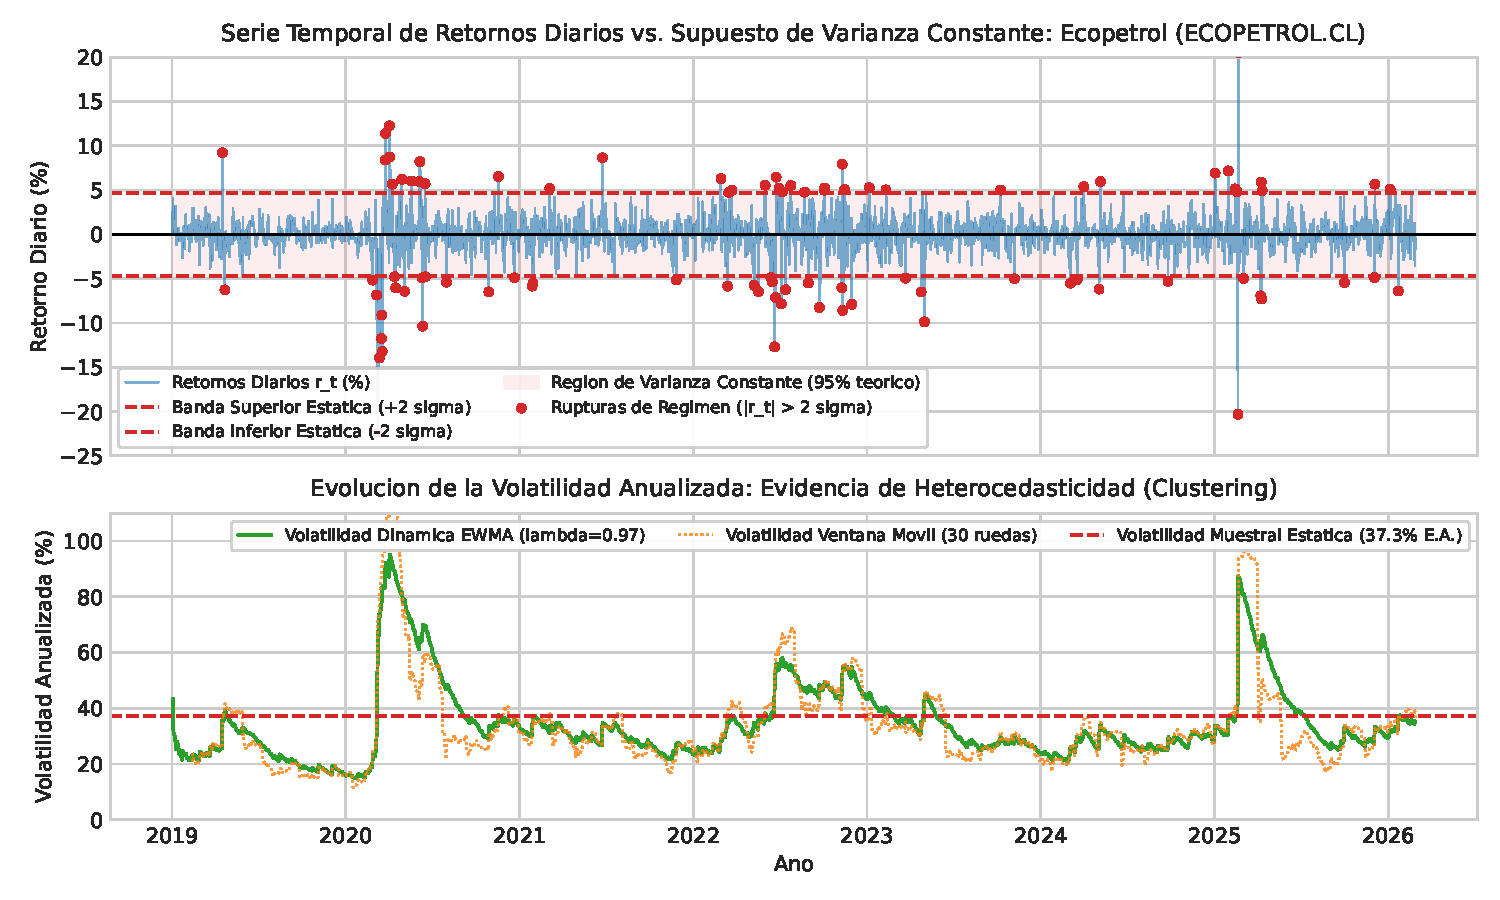
\includegraphics[width=0.88\textwidth,height=0.74\textheight,keepaspectratio]{grafica_retornos_varianza_constante.pdf}
  \end{center}
\end{frame}

% SLIDE 27: DISCUSION DEL PROBLEMA DE VARIANZA CONSTANTE
\begin{frame}{26. Diagnostico del Supuesto de Varianza Estatica}
  La serie de retornos diarios de Ecopetrol (2019--2026) ilustra una limitacion practica:
  \vspace{0.3cm}
  \begin{itemize}
    \item Si la matriz $C$ se estima mediante la covarianza muestral estatica tradicional, se asume que la varianza permanece fija e inalterable en el tiempo ($\pm 2\sigma$ constante).
    \vspace{0.2cm}
    \item Sin embargo, las series financieras exhiben conglomerados de volatilidad: periodos de calma alternados con explosiones de riesgo e incertidumbre.
    \vspace{0.2cm}
    \item Los retornos reales perforan frecuentemente las bandas gaussianas teoricas de dos desviaciones estandar en periodos criticos (marzo 2020 y mediados de 2022).
    \vspace{0.2cm}
    \item Esto genera inercia muestral: el modelo tarda meses en reconocer un aumento en la volatilidad si promedia dias antiguos por igual.
  \end{itemize}
\end{frame}

% SLIDE 28: CONTROL PREDICTIVO POR MODELO (WALK-FORWARD)
\begin{frame}{27. Solucion Algoritmica: Control Predictivo por Modelo (MPC)}
  Para corregir la inercia sin alterar la formulacion cuadratica determinista:
  \vspace{0.3cm}
  \begin{itemize}
    \item 1. En cada fecha de rebalanceo trimestral $t_k$, se recalculan los parametros deterministas $P$ y $C$ empleando filtros adaptativos de memoria reciente (como EWMA con $\lambda=0.97$ o estimadores de semi-covarianza a la baja).
    \vspace{0.2cm}
    \item 2. Se resuelve el sistema KKT determinista para las $M=3$ etapas futuras de planeacion.
    \vspace{0.2cm}
    \item 3. Se implementa en el portafolio real unicamente la primera asignacion de decisiones $U_0^*$.
    \vspace{0.2cm}
    \item 4. Al llegar el siguiente trimestre, la ventana de observacion avanza un paso y el procedimiento se repite con las nuevas condiciones del mercado.
  \end{itemize}
\end{frame}

% SLIDE 29: CONCLUSIONES
\begin{frame}{28. Conclusiones para la Teoria y Practica de la Optimizacion}
  \begin{itemize}
    \item 1. Rigor y Unicidad Global: La formulacion multiperiodo como Programa Cuadratico estrictamente convexo garantiza que las condiciones KKT caracterizan de forma necesaria y suficiente el unico punto optimo global.
    \vspace{0.3cm}
    \item 2. Riqueza de la Informacion Dual: El vector de multiplicadores proporciona una radiografia completa de la sensibilidad del sistema:
    \begin{itemize}
      \item $\Lambda$ mide la tasa marginal de productividad intertemporal del presupuesto.
      \item $Y$ cuantifica el costo de exclusion de activos poco eficientes.
      \item $Z$ senala a los comites de riesgo que restricciones regulatorias estan limitando el desempeno potencial.
    \end{itemize}
    \vspace{0.3cm}
    \item 3. Eficiencia Numerica: Los solucionadores modernos de optimizacion convexa (como OSQP y Clarabel) resuelven este sistema en menos de 10 milisegundos, permitiendo auditorias de sensibilidad continuas en tiempo real.
  \end{itemize}
\end{frame}

% SLIDE 30: CIERRE
\begin{frame}
  \begin{center}
    \vspace{1.5cm}
    {\Large Preguntas y Discusion}
    
    \vspace{1.0cm}
    Juan Mario Delgado Molina\\
    Curso de Optimizacion Lineal y Convexa
  \end{center}
\end{frame}

\end{document}
